%
% File acl2018.tex
%
%% Based on the style files for ACL-2017, with some changes, which were, in turn,
%% Based on the style files for ACL-2015, with some improvements
%%  taken from the NAACL-2016 style
%% Based on the style files for ACL-2014, which were, in turn,
%% based on ACL-2013, ACL-2012, ACL-2011, ACL-2010, ACL-IJCNLP-2009,
%% EACL-2009, IJCNLP-2008...
%% Based on the style files for EACL 2006 by 
%%e.agirre@ehu.es or Sergi.Balari@uab.es
%% and that of ACL 08 by Joakim Nivre and Noah Smith

\documentclass[11pt,a4paper]{article}
\usepackage[hyperref]{acl2018}
\usepackage{times}
\usepackage{latexsym}
\usepackage{color}
\usepackage{url}
\usepackage{graphicx}
\graphicspath{ {./Figures/} }

\aclfinalcopy % Uncomment this line for the final submission
%\def\aclpaperid{***} %  Enter the acl Paper ID here

%\setlength\titlebox{5cm}
% You can expand the titlebox if you need extra space
% to show all the authors. Please do not make the titlebox
% smaller than 5cm (the original size); we will check this
% in the camera-ready version and ask you to change it back.

\newcommand\BibTeX{B{\sc ib}\TeX}

\title{Classifying Job Review Helpfulness Using Convolutional Neural Networks}

\author{Ryan Delgado \\
	datascience@berkeley.edu / W266: NLP with Deep Learning \\
	{\tt rmdelgad2013@berkeley.edu}
}

\date{}

\begin{document}
	\maketitle
	\begin{abstract}
	I introduce a novel dataset of job reviews scraped from company review pages on Glassdoor.com, and report on experiments of classifying the helpfulness  of reviews using an SVM with bigram word counts and a Convolutional Neural Network (CNN), with the CNN model achieving \textcolor{blue}{(significantly/marginally/tbd)} better accuracy scores than the baseline model at this classification task. I also experiment with using pre-trained and untrained word embeddings in the CNN model, and observe that the pre-trained embeddings \textcolor{blue}{(outperforms/underperforms/tbd)} the untrained embeddings. 
	\end{abstract}
	
	
	\section{Introduction}
	Glassdoor is a widely used website that allows current and former employees to post anonymous ratings about their experience working at any company registered on the site. This allows potential employees to research companies before beginning employment or the interview process, and provides employers the opportunity to obtain candid feedback about their work environment. Reviewers are asked to score companies overall on a 5-star scale, and offered the opportunity to write about the positive and negative aspects of the company. Glassdoor has only a simple content approval process, so individuals seeking quality reviews may have to read through tens or even hundreds of reviews in order to gather enough information about a future employer. Glassdoor provides a peer review system through the use of its "Helpful" button, which allows review readers to rate any review they come across. However, no current standards exist to guide users regarding what "Helpful" may mean in this context. Determining commonalities between those reviews indicated as "Helpful" could aid in guiding users toward those reviews that may offer them the most useful information.
		
	This paper introduces a novel dataset of job reviews scraped from Glassdoor, and explores using Machine Learning models to classify the helpfulness of job reviews. Almost 260,000 English-language reviews were scraped from the companies in Glassdoor's Top 100 Best Places to Work of 2018. I try two different models to classify reviews: 1. A baseline machine learning model based on bigram counts of the reviews and a Support Vector Machine (SVM) model 2. A Convolutional Neural Network (CNN) model. In the CNN model, I experiment with using static and non-static pre-trained word embeddings and also word embeddings trained from scratch. The CNN models improves \textcolor{blue}{(significantly/marginally/tbd)} on the baseline model.
	
	\section{Background}
	
	\subsection{Dataset and Task}
	The data used in this experiment was compiled by scraping reviews and Helpfulness scores from Glassdoor. Specifically, the reviews are of companies that were ranked in the Top 100 Best Places to Work of 2018. Each review contains both 'Pros' and 'Cons' reviews, so I combined these two sub-reviews were concatenated into one review. The helpfulness score for each review was binarized to 1 if the review had a helpfulness score of at least 1, 0 otherwise. Each review and score pair is an observation in the dataset, and predicting review helpfulness is framed as a binary classification problem. Figure 1 shows a histogram of the word counts. Figure 2 shows a word cloud of all of the reviews. Table 1 lists descriptive statistics about the dataset.
	
	\begin{figure}[h]
	\begin{center}
		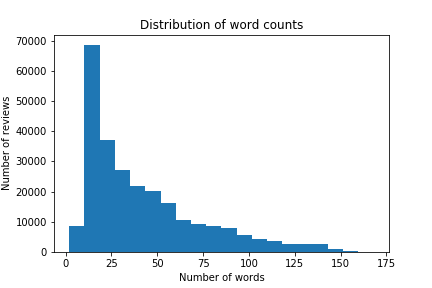
\includegraphics[scale=0.5]{wordcounts}
		\caption[scale=0.75]{Distribution of the word counts across the Glassdoor reviews.}
	\end{center}
	\end{figure}

	\begin{figure}[h]
	\begin{center}
		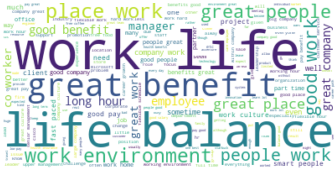
\includegraphics[scale=0.75]{wordcloud}
		\caption[scale=0.75]{Word cloud of the reviews.}
	\end{center}
	\end{figure}

	\begin{table}[h]
	\begin{center}
	\begin{tabular}{|l|l|}
		\hline \textbf{Statistic} & \textbf{Value} \\ \hline
		Num of Observations & 259,317 \\
		Vocab Size & 110,897 \\
		Avg Review Length & 41 \\
		Max Review Length & 168 \\
		Min Review Length & 2 \\
		Avg Helpful Review Length & 57 \\
		Avg Not Helpful Review Length & 35 \\
		Pct Helpful Reviews & 71.24\% \\
		Pct Unhelpful Reviews & 28.76\% \\
		\hline
	\end{tabular}
	\caption[scale=0.75]{Descriptive Statistics on the Dataset.}
	\end{center}
	\end{table}

		
	\subsection{Baseline SVM Model}
	Wang and Manning \cite{Wang} investigate two common baseline models for text classification: Multinomial Naive Bayes (MNB) and a Support Vector Machine (SVM). They train and test these models over four different datasets with varying input lengths, and find that MNB perform better at classifying snippets and short sentences, while SVMs outperforms at classifying longer documents like movie reviews. They also find that using bigrams word counts in sentence classification improves classification accuracy. Based on these results, I decided to use an SVM with a linear kernel and bigram word count features as my baseline model. I chose the SVM because job reviews tend to be longer than just snippets, with an average review length of 41 words. Observations were divided into train and test datasets, which were used to train and evaluate the model. The baseline model was trained using Stochastic Gradient Descent and achieves an accuracy score on the test set of \textbf{73.98\%}.	
			
	\subsection{CNN Model}
	CNNs have shown exceptional results in text classification tasks. Kim \cite{Kim} showed that CNN variations improved on the state of the art in 4 out of 7 sentence classification tasks, and still achieved excellent results compared to other neural network models and classical models with hand-coded features. Architecture of Kim's model:
	
	\begin{enumerate}
		\item An embedding layer, with one k-dimensional vector for each word
		\item A single 1-dimensional convolutional layer with multiple features and window sizes
		\item A max-over-time pooling layer
		\item A fully-connected softmax layer that produces the probabilities among the labels
	\end{enumerate}

	Kim's experiments included model variants where the embedding layer used pre-trained by Mikolov et al.'s \cite{word2vec} Word2Vec algorithm, and shows that these achieve consistently better results than randomly initializing the embeddings and tuning them as part of training. Zhang and Wallace \cite{Zhang} also find that using pre-trained word vectors enhances classification performance, and show that using either Word2Vec or GloVe \cite{Pennington} embeddings results in similar performance. They do show, however, that allowing the embedding layer to be tuned during training uniformly outperforms CNN variants whether the embedding layer is held static. They also postulate that learning embeddings from scratch may have better results in datasets with many observations. Since my dataset is fairly large, I'll experiment with both using pre-trained GloVe vectors in the embedding layer, and a randomly initialized embedding layer trained from scratch.
	
	Kim \cite{Kim} experiments with many different filter sizes and feature maps in the convolutional layer, but Zhang \cite{Zhang} suggests that optimal filter sizes for datasets with longer text is likely greater than 10. Their example was the Amazon Customer Reviews dataset from Hu and Liu \cite{Hu} (denoted as the "CR" dataset in \cite{Zhang}), which has a max review length of 105. Since the max review length in my dataset is 165 words, I'll experiment with filter sizes up to 30. Zhang \cite{Zhang} also states that different feature map sizes can result in better performance, irrespective of the sentence length. I'll experiment with feature map sizes of 50, 100, and 200.
	
	Zhang and Wallace \cite{Zhang} experimented with different pooling strategies, and found that that 1-max pooling consistently outperforms alternative strategies like k-max pooling and average pooling. Additionally, they experiment with different dropout rates to regularize their CNN models, and find that varying the dropout rate does not materially affect performance, except for dropout rates above 0.7 which almost uniformly perform poorly. Thus I will only use 1-max pooling and a dropout rate of 0.5 in my experiments.

	\textcolor{blue}{Note for the W266 instructors: I'll modify this section to the past tense after I've finished training the CNN models.}
	
	\section{Results}
	\textcolor{blue}{In this section I'll report the empirical results of the CNN variants, and compare them to the baseline. I'll discuss the results from the variations in standard CNN model hyperparameters (i.e. feature map size, filter size) and hypothesize why certain configurations led to better performance.}

	\subsection{Pre-trained vs Untrained Embeddings}
	\textcolor{blue}{In this subsection I'll compare the results between the best pre-trained and untrained embedding layer models. If there is a significant difference, I'll examine cases where one model was correct and the other incorrect, and hypothesize why this occurred.}
	
	\subsection{Error Analysis}
	\textcolor{blue}{In this section I'll focus on the best CNN model, and examine instances where it got the prediction \textit{very} wrong, i.e. it predicted Helpful with a high probability but it was actually not labeled Helpful. I'll discuss why this happened, and talk about what improvements could be made to the model to potentially improve performance.}
	
	\section{Conclusion}
	\textcolor{blue}{I'll summarize my findings and wrap up in this section.}

	
	\bibliographystyle{plain}
	\bibliography{glassdoor}

	
	
\end{document}
